%! Author = joels
%! Date = 27/01/2022

\section{JIT Compiler}
\begin{itemize}[topsep=0pt]
    \itemsep -0.2em
    \item Effizientere Ausführung als Interpretation
    \item Bytecode direkt in nativen Prozessor-Code übersetzen und ausführen
    \item Nicht unbedingt alles, sondern nur Performance-kritische Teile
    \item z.B. Häufig ausgeführter Code (>= 50 mal)
\end{itemize}

\textbf{Profiling:}
\begin{itemize}[topsep=0pt]
    \itemsep -0.2em
    \item Interpreter zählt Ausführung gewisser Code-Teile
    \SubItem{Methoden}
    \SubItem{Traces (Code-Pfade)}
    \item Falls häufig ausgeführt: JIT für den Teil anwerfen
\end{itemize}

\subsection{Intel 64 Architektur}
\begin{itemize}[topsep=0pt]
    \itemsep -0.2em
    \item Instruktionen benutzen Register
    \item 14 allgemeine register für Ganzzahlen
    \SubItem{RAX, RBX, RCX, RDX, RSI, RDI, R8..R15}
\end{itemize}

\subsection{Arithmetische Instruktionen}
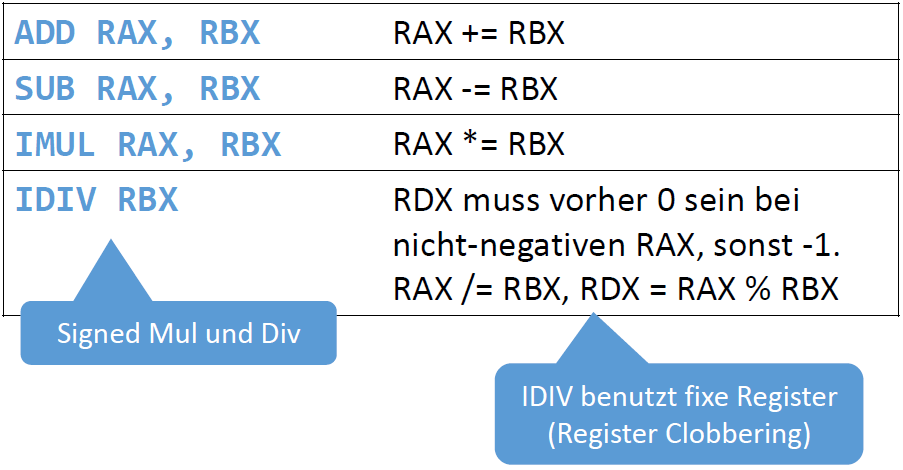
\includegraphics[width=0.8\linewidth]{arithmetische_instruktionen}

\subsubsection{IDIV vorbereiten}
\textbf{CDQ:} Vorzeichenbehaftete Konversion von RAX nach RDX:RAX (Convert to Quad Word)
\begin{lstlisting}
// Rechnung: (x - 1) / 2
// x sein in RAX
MOV RBX, 1
SUB RAX, RBX // RAX = x - 1
MOV RBX, 2
CDQ // RDX für IDIV vorbereiten
IDIV RBX // RAX = (x - 1) / 2
// Resultat in RAX
\end{lstlisting}

\subsection{Register Allokation}
Passende register für Code-Fragmente bestimmen:
\begin{itemize}[topsep=0pt]
    \itemsep -0.2em
    \item Registerauswahl Hängt von vorherigen Instruktionen ab
    \item Durch Instruktion werden register frei oder belegt
\end{itemize}

\subsubsection{Lokale register-Allokation}
\begin{itemize}[topsep=0pt]
    \itemsep -0.2em
    \item Für Ausdrucksauswertung (Evaluation Stack)
    \item Evaluation Stack Einträge auf Register abbilden $\rightarrow$ Register Stack
\end{itemize}

\textbf{Vorgehen:}
\begin{itemize}[topsep=0pt]
    \itemsep -0.2em
    \item Cross Compiler führt Stack an belegten Register
    \SubItem{Register Stack entspricht also dem Evaluation Stack}
    \item Pro übersetzte Byte-Code Instruktion wird der Stack nachgeführt
\end{itemize}

\textbf{Register Clobbering}
\begin{itemize}[topsep=0pt]
    \itemsep -0.2em
    \item IDIV überschreibt RAX und RDX als Seiteneffekt
    \item Sichere benötigte Werte von RAX und RDX vor IDIV
\end{itemize}

\subsubsection{Globale Register-Allokation}
\begin{itemize}[topsep=0pt]
    \itemsep -0.2em
    \item Variablen in Register speichern (in bestimmten Abschnitten)
    \SubItem{Insbesondere Locals und Params}
    \item Deutlich schneller als Speicherzugriffe
    \item Idee: Aktuelle Allokation merken
\end{itemize}

\subsubsection{Intel Branches}
\begin{itemize}[topsep=0pt]
    \itemsep -0.2em
    \item Bedingte Sprünge basierend auf Condition Code
    \item Condition Code aus vorherigem Vergleich
    \SubItem{Zuerst: CMP RAX, RBX und dann JE target}
\end{itemize}

\subsection{Implementation}
\begin{lstlisting}
switch (opCode) {
    // Load Constant
    case LDC -> {
        var target = acquire();
        var value = (int)instruction.getOperand();
        assembler.MOV_RegImm(target, value);
        push(target);
    }

    // Load
    case LOAD -> {
        X64Register reg;
        var index = (int)instruction.getOperand();
        var nofParams = allocation.parameters.size();
        var nofLocals = allocation.locals.size();
        if (index <= nofParams) {
            reg = allocation.parameters().get(index - 1);
        } else if (index <= nofParams + nofLocals) {
            reg = allocation.locals().get(index - 1 - nofParams);
        }
        push(reg);
    }

    // Store
    case STORE -> {
        var source = pop();
        // Check, ob locals oder params (wie bei load)
        var target = allocation.locals().get(index - 1 - nofParams);
        assembler.MOV_Regreg(target, source);
        release(source);
    }

    // ISub
    case ISUB -> {
        var subtrahend = pop();
        var minuend = pop();
        var difference = acquire();
        assembler.MOV_RegReg(difference, minuend);
        assembler.MOV_RegReg(difference, subtrahend);
        release(subtrahend);
        release(minuend);
        push(difference);
    }

    // IDiv
    case IDIV -> {
        reserve(RAX);
		reserve(RDX);
		forceStack(1, RAX);
		var divisor = pop();
		pop();
		assembler.CDQ();
		assembler.IDIV(divisor);
		push(RAX);
		release(divisor);
		release(RDX);
    }

    // Any Compare Operation
    case CMPEQ -> {
        var right = pop();
		var left = pop();
		assembler.CMP_RegReg(left, right);
		previous = opCode;
		release(left);
		release(right);
    }

    // Verzweigung (Jump)
    case if_true -> {
        var offset = (int)instruction.getOperand();
        var target = code[position + 1 + offset];
        var label = labels.get(target);
        matchAllocation(label);
        switch(previous) {
            case CMPEQ -> assembler.JE_Rel(label);
            case CMPNE -> assembler.JNE_Rel(label);
            case ICMPLT -> assembler.JL_Rel(label);
            case ICMPLE -> assembler.JLE_Rel(label);
            case ICMPGT -> assembler.JG_Rel(label);
            case ICMPGE -> assembler.JGE_Rel(label);
            default -> throw new AssertionError("Unsupported operand before if_true in JIT compiler");
        }
    }
}
\end{lstlisting}